\documentclass{beamer}

\usepackage[utf8]{inputenc}

\usepackage{graphicx}
\title{Glass Classification}
\author{Patrick Bettermann}
\date{16.12.2020}



\begin{document}

\frame{\titlepage}

\begin{frame}
\frametitle{}
  \begin{columns}[T]
    \begin{column}{.5\textwidth}
     \begin{block}{Is it used for?}
     	\begin{itemize}
     	\item{buildings?}
     	\item{cars?}
     	\item{tableware?}
     	\end{itemize}
     \end{block}
     \begin{block}{Furthermore}
     	is it processed in a special 
     	way?
     \end{block}
    \end{column}
    \begin{column}{.5\textwidth}
    \begin{block}{What type of glass 
    is this?}
    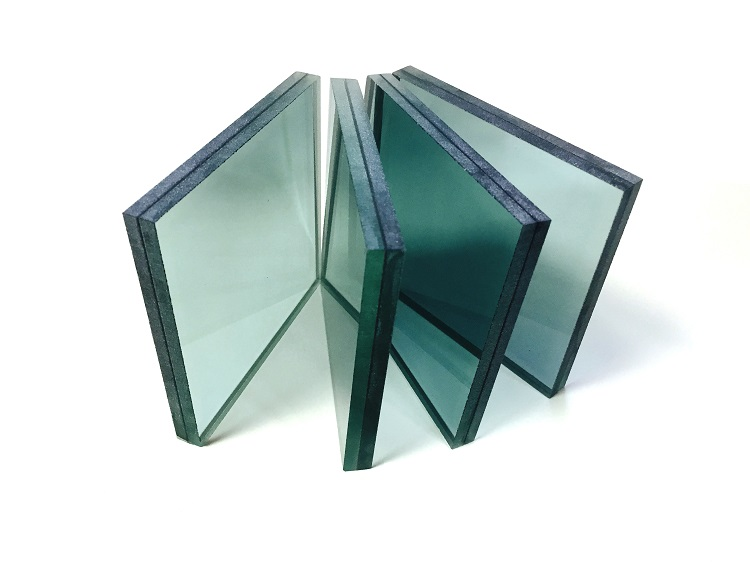
\includegraphics[]{glass.jpg}
    \end{block}
    \end{column}
  \end{columns}
\end{frame}

\begin{frame}
\frametitle{Dataset}
\begin{itemize}
\item{\url{https://www.kaggle.com/uciml/glass}}
\item{only 214 entries of different types (7) of glass}
\item{glass characterized by \\
- RI: refractive index\\
- Na: Sodium (weight percent in corresponding oxide)\\
- Si: Silicon\\
 ...}
\item{which are therefore correlated}
\end{itemize}
\end{frame}

\begin{frame}
\frametitle{Prepare data}
\begin{itemize}
\item{input: csv file $\rightarrow$ .txt}
\item{70\% of the entries are type 1 and 2 \\
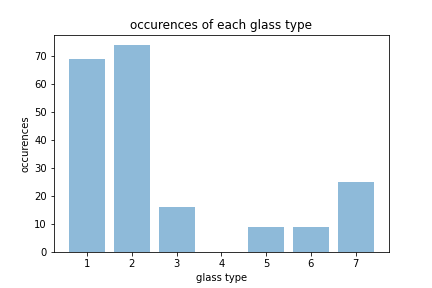
\includegraphics[scale=0.35]{count.png}}
\item{cleaning: delete entrie if value differs by $\pm \bar{x}$\\
- zero values not counted}
\end{itemize}
\end{frame}

\begin{frame}
\frametitle{Prepare data - cleaning}
\begin{columns}[T]
    \begin{column}{.5\textwidth}
     \begin{block}{}
     \end{block}
     \begin{block}{Ba: Barium}
	   	- 176 of 214 values empty\\
     	- some outliers\\
     	- mostly present in type 7
        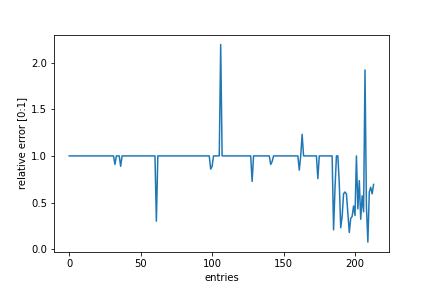
\includegraphics[scale=0.4]{
        figBa.png}
     \end{block}
    \end{column}
    \begin{column}{.5\textwidth}
    \begin{block}{Na: Natrium}
    - no outliers \\
    - present in all types of glass
       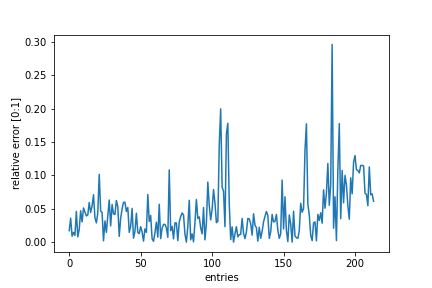
\includegraphics[scale=0.4]
       {figNa.png}
    \end{block}
    \end{column}
  \end{columns}
\end{frame}

\begin{frame}
\frametitle{Random Forests}
\begin{itemize}
\item{reliant model}
\item{key ideas:\\ - randomnes of the tree construction\\ - many randomly constructed trees should compensate for errors \\ - random and independant data selection}
\item{can overfit}
\end{itemize}
\end{frame}

\begin{frame}
\frametitle{Encoding}
\begin{itemize}
\item{no encoding needed}
\item{only seperation of data and labels is performed}
\end{itemize}
\end{frame}

\begin{frame}
\frametitle{Tuning}
- parameters: max. depth, number of trees, how to split the tree, ...
\begin{columns}[T]
    \begin{column}{.5\textwidth}
     \begin{block}{}
     \end{block}
     \begin{block}{max. depth = 2}
     	- capped at 65\%\\
        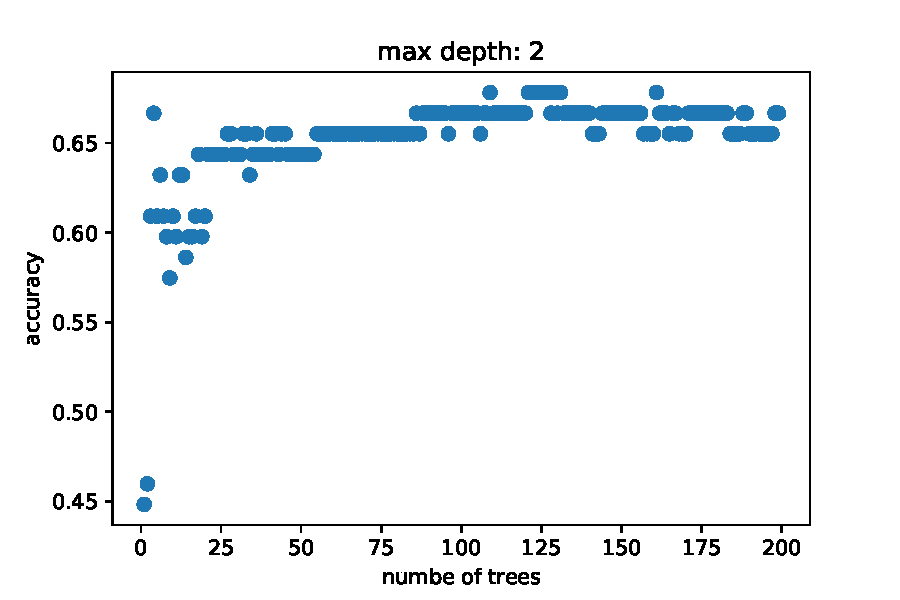
\includegraphics[scale=0.4]{
        result2.pdf}
     \end{block}
    \end{column}
    \begin{column}{.5\textwidth}
    \begin{block}{max. depth = 4}
    - up to 79\% accuracy\\
       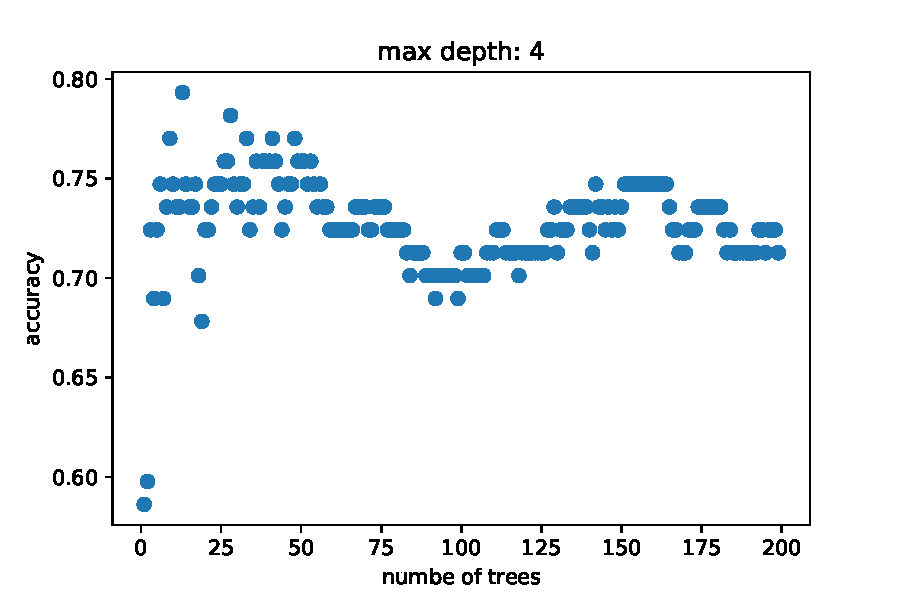
\includegraphics[scale=0.4]
       {result4.pdf}
    \end{block}
    \end{column}
  \end{columns}
\end{frame}

\begin{frame}
\frametitle{Train/Validation}
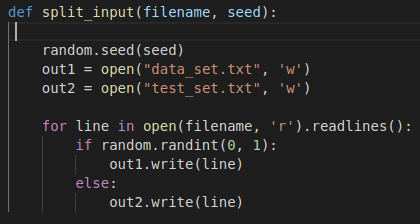
\includegraphics[scale=0.6]
       {splitinput.png}
\begin{itemize}
\item{problem: data set is very small \\ now it's even smaller}
\end{itemize}
\end{frame}

\begin{frame}
\frametitle{Results}
\begin{itemize}
\item{best parameters: \\
number of trees = 13\\
max. depth = 4\\
$\rightarrow$ result: 79\% of predictions are correct}
\item{only 200 entries $\rightarrow$ trees don't need to be complex}
\end{itemize}
\end{frame}

\begin{frame}
\frametitle{Discussion}
\begin{itemize}
\item{check for overfitting is missing}
\item{how to handle zero values?}
\item{Are there better methods to find outliers than difference to mean?}
\item{Maybe leave-one-out-cross-validation might work since the data set is so small?} 
\end{itemize}
\end{frame}

\begin{frame}
\frametitle{Code - evaluation}
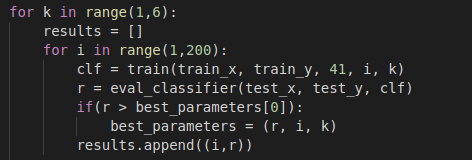
\includegraphics[scale=0.7]
       {code1.png}
\end{frame}

\begin{frame}
\frametitle{Code - get an idea of the data}
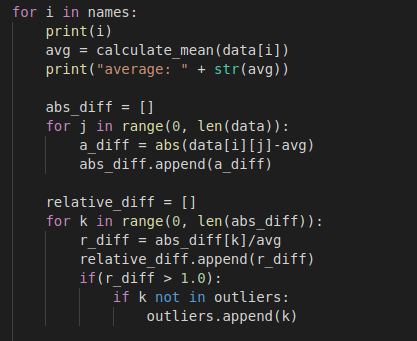
\includegraphics[scale=0.65]
       {code2.png}
\end{frame}

\end{document}
